\section{Goals}

\subsection{Goal 1}

\begin{enumerate}
    \item {\bf When the ACC is active, vehicle speed shall be controlled automatically to maintain a time gap to the forward vehicle or maintain a set speed.}
    \begin{enumerate}[label*=\arabic*]
        \item The system shall maintain a time gap to the forward vehicle
        \begin{enumerate}[label*=\arabic*]
            \item The system shall have a minimum selectable time gap value for all speeds
            \item The system shall provide at least one time gap value in the range of 1.5 seconds to 2.2 seconds
            \item The system shall align to the minimum time gap limit
            \item The system shall adjust the time gap to achieve the limit within an appropriate time, if the time gap temporarily falls below the limit
        \end{enumerate}
        \item The system shall maintain a set speed
        \begin{enumerate}[label*=\arabic*]
            \item The system shall align the subject speed to a set speed
        \end{enumerate}
        \item The system shall make the transition between the two modes automatically
        \begin{enumerate}[label*=\arabic*]
            \item{The system shall select the mode with the lowest speed}
        \end{enumerate}
        \item{The system shall be able to determine the speed of the subject vehicle}
        \begin{enumerate}[label*=\arabic*]
            \item{The measured speed shall be the same as the physical speed}
        \end{enumerate}
        \item{The system shall have target discrimination}
        \begin{enumerate}[label*=\arabic*]
            \item{The system shall select the forward vehicle in the subject’s lane, if there are more than one forward vehicle on the road}
        \end{enumerate}
        \item{The system shall have detection ranges}
        \begin{enumerate}[label*=\arabic*]
            \item{The measured range shall be the same as the physical range}
            \item{The system shall measure the range between the forward and the subject vehicles, if a forward vehicle is present within range A}
            \item{The system shall detect the presence of a vehicle within range B}
            \item{The system shall increase clearance and/or inhibit automatic acceleration if a vehicle is detected within range B}
        \end{enumerate}
        \item{The system shall have curve capabilities}
        \begin{enumerate}[label*=\arabic*]
            \item The system shall allow following of vehicles on curves and straight roads
        \end{enumerate}
    \end{enumerate}
\end{enumerate}

\begin{figure}[H]
    \centering
    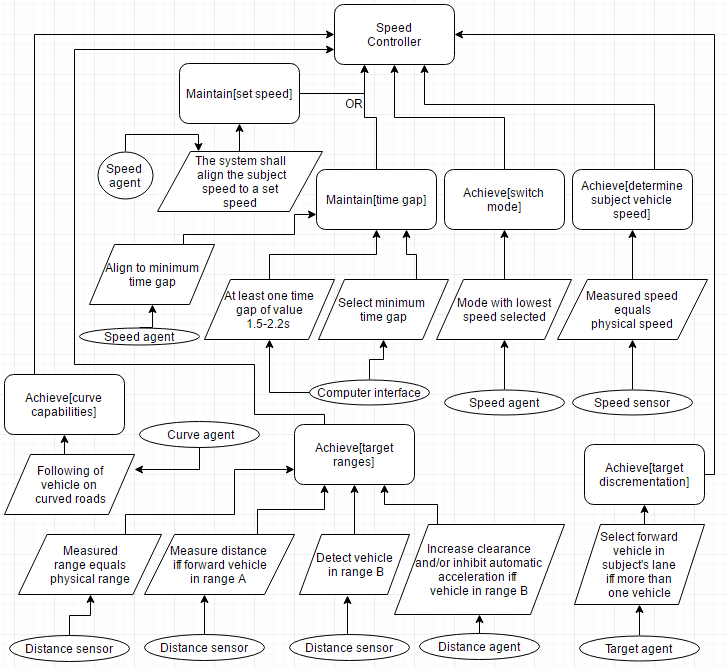
\includegraphics[width=\textwidth]{images/goal1_graph}
    \caption{Refinement graph for goal 1}
    \label{fig:graph_1}
\end{figure}

\vspace{1.5cm}

\subsection{Goal 2}

\begin{enumerate}
    \item {\bf The ACC-system is turned off}
    \begin{enumerate}[label*=\arabic*]
        \item Off state can be forced automatically from either Stand-by or Active state by failure reaction.
        \item Off state can be set manually from either Stand-by or Active state by a manual switch.
        \item Off state can be set manually and/or automatically after self test from either Stand-by or Active state.
    \end{enumerate}

    \item {\bf The ACC-system is in stand-by state}
    \begin{enumerate} [label*=\arabic*]
        \item Stand-by state can be activated manually and/or automatically from self test, from off state.
        \item Stand-by state can be activated by a human interaction with the breaks
        \begin{enumerate}[label*=\arabic*]
            \item Braking by the driver shall deactivate ACC function at least if the driver initiated brake force demand is higher than the ACC initiated brake force
            \item Type 1a and 2a ACC systems can transposition to ACC-stand-by from active state if the driver depresses the clutch pedal
        \end{enumerate}
    \end{enumerate}
    \item {\bf The ACC-system is in active state}
    \begin{enumerate}[label*=\arabic*]
        \item Active state can be activated only from Stand-by state via user interaction.
        \item Active state should switch between ACC speed control and ACC time gap control.
    \end{enumerate}
\end{enumerate}


\begin{figure}[H]
    \centering
    \includegraphics[width=\textwidth]{images/goal2_graph.png}
    \caption{Refinement graph for goal 2}
    \label{fig:graph_2}
\end{figure}



\subsection{Goal 3}

\begin{enumerate}
    \item{\bf Manual clutch operation}
    \begin{enumerate}[label*=\arabic*]
        \item{ACC shall either be suspended or transition to stand-by after use of clutch}
    \end{enumerate}
    \item{\bf No manual clutch operation, no active brake controls}
    \begin{enumerate}[label*=\arabic*]
        \item{}
    \end{enumerate}
    \item{\bf Manual clutch operation, active brake control}
    \begin{enumerate}[label*=\arabic*]
        \item{ACC shall either be suspended or transition to stand-by after use of clutch}
        \item{Brake control can be continued during use of clutch}
        \item{Driver should be informed clearly about potential conflict between brake and engine idle control}
    \end{enumerate}
    \item{\bf Active brake control}
    \begin{enumerate}[label*=\arabic*]
        \item {The ACC system can apply the brakes automatically}
        \item {If the power demand of the driver is greater than that of the ACC system automatic breaking shall be disengaged with an immediate brake force release}
        \item {Brake light shall be illuminated when automatic braking is applied}
        \begin{enumerate}[label*=\arabic*]
            \item {The lights shall be illuminated within 100 ms}
            \item {To prevent irritating brake light flickering, the brake light may remain on for a reasonable time after the ACC initated braking has ended}
        \end{enumerate}
    \end{enumerate}   
    \item{\bf ACC type 1 should react to failed subsystems}
    \begin{enumerate}[label*=\arabic*]
        \item{Engine failure}
        \begin{enumerate}[label*=\arabic*]
            \item{If the engine fails the ACC engine control mode should be relinquished}    
        \end{enumerate}
        \item{Gearbox failure}
        \begin{enumerate}[label*=\arabic*]
            \item{If the gearbox fails the ACC control mode and engine mode should be relinquished}    
        \end{enumerate}
        \item{Detecting and ranging sensor failure}
        \begin{enumerate}[label*=\arabic*]
            \item{If detecting and ranging sensor fails the ACC should maintain same strategy as the time before fault}
            \item{The system should be switched off immediately after driver intervention by brake or accelerator pedal or ACC off switch}
            \item{ACC engine control mode should be relinquished}
        \end{enumerate}
        \item{ACC controller failure}
        \begin{enumerate}[label*=\arabic*]
            \item{ACC control mode should be relinquished}
        \end{enumerate}
    \end{enumerate}
    \item{\bf ACC type 2 should react to failed subsystems}
    \begin{enumerate}[label*=\arabic*]
       \item{Engine failure}
       \begin{enumerate}[label*=\arabic*]
           \item{Should maintain braking as required at least for the actual / current braking maneuver}
           \item{ACC engine control mode should be relinquished}
       \end{enumerate}
       \item{Brake system failure}
       \begin{enumerate}[label*=\arabic*]
           \item{ACC control mode and engine control mode should be relinquished}
       \end{enumerate}
       \item{Detecting and ranging sensor failure}
       \begin{enumerate}[label*=\arabic*]
           \item{Should initiate a controller strategy starting with the last valid braking command}
           \item{The system should be switched off immediately after driver intervention by brake or accelerator pedal or ACC off switch}
           \item{ACC engine control mode should be relinquished}
       \end{enumerate}
       \item{ACC controller failure}
       \begin{enumerate}[label*=\arabic*]
           \item{ACC control mode should be relinquished}
       \end{enumerate}
    \end{enumerate}
\end{enumerate}
\newpage

\begin{figure}[H]
    \hspace*{-4cm}
    \centering
    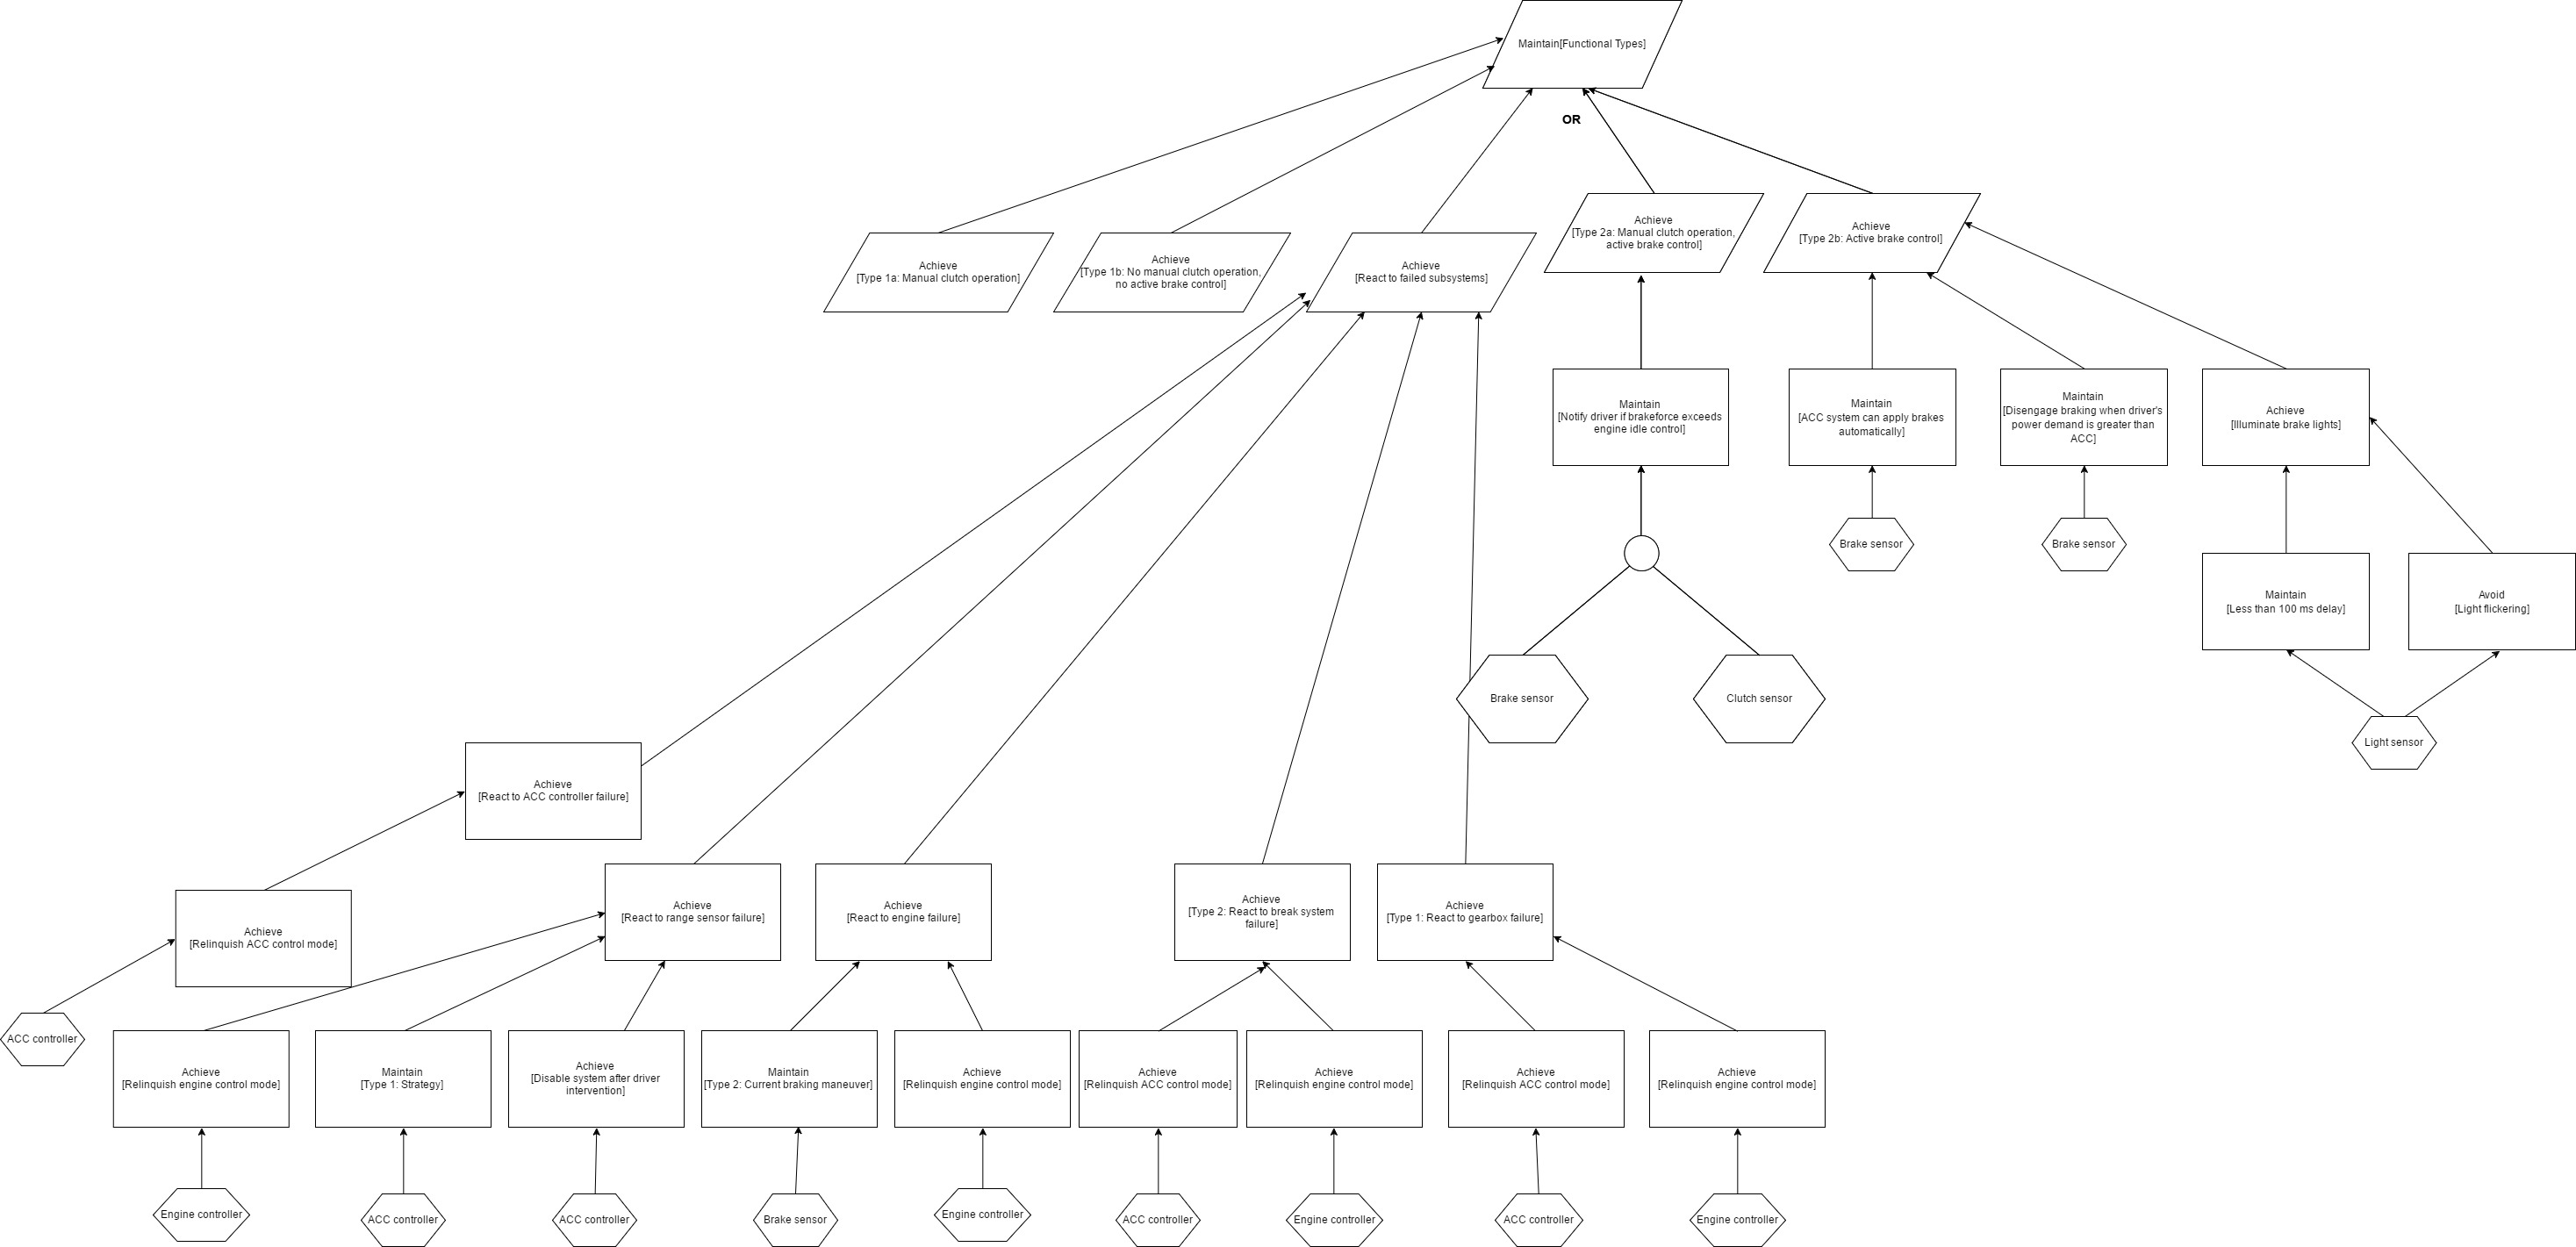
\includegraphics[scale=0.180]{images/RefinementGraph}
    \caption{Refinement graph for goal 3}
    \label{fig:graph_3}
\end{figure}

%\begin{sidewaysfigure}
%    \centering
%    \includegraphics[width=\textwidth]{images/goal3_graph}
%    \caption{Refinement graph for goal 3}
%    \label{fig:my_label}
%\end{sidewaysfigure}


%\includegraphics[width=\textwidth,height=\textheight]{images/goal3_graph}

